\vspace*{.2in}
\begin{figure}[htb]
\begin{center}
\leavevmode
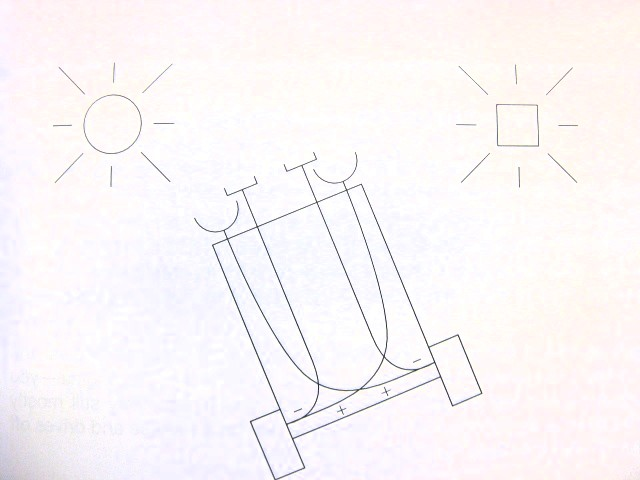
\includegraphics[width=100mm]{IMG_0004.JPG}
\end{center}
\caption{Braitenberg's Light/Sound Finder~\cite{RoboticExplorations} }
\label{fig:LightSoundFinder}
\end{figure}

Implementing a robot that has only one sensor is relatively simple compared to implementing a robot that uses multiple sensors in conjunction with each other.  However, using multiple sensors allows different sensors to cover other sensors week spots.  Every single sensor has some week spot.  The standard light sensor can not pick up dark objects due to the light reflected.   In this case you can think of bright surfaces such as snow as reflecting the majority of light.  Furthermore, dark surfaces have the opposite effect, this is because they absorb light.  As a result of anything dark absorbing light, the sensor no longer has as much reflected light to measure.  As such, this generally shows that every sensor has its own weakness furthermore, different sensors can compensate for each-others weaknesses.\\

Figure~\ref{fig:LightSoundFinder} is very similar to figure~\ref{fig:LightFinder}, they both use the same style light sensor.  However, figure~\ref{fig:LightSoundFinder} uses an additional type of sensor.  The half square boxes represent a sound receiver.  The sound senors are set up in a different way than the light sensors.  Each sound sensor connects to the motor on its side.  In addition, looking at the connection between the sound sensor and motor we see that there is a minus sign.  As we can see, the stronger the sound the stronger the signal that the sound sensor produces.  However, the minus implies that it is a subtractive signal, or otherwise known as a negative signal.  This will subtract from the positive signal feedback from the light sensor.  In turn, this causes the wheel to slow down.  However, since the sound sensor connects to the motor on the same side it will turn towards the sound given that the signal is strong enough to over ride the sound sensors.\cite{RoboticExplorations}\\



\vspace*{.2in}
\begin{figure}[h!]
\begin{center}
\leavevmode
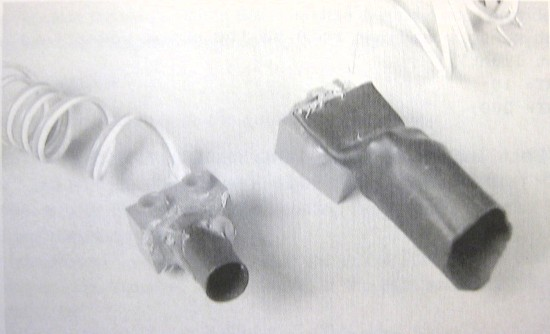
\includegraphics[width=100mm]{IMG_0005.JPG}
\end{center}
\caption{Focusing Light Sensor~\cite{RoboticExplorations} }
\label{fig:LightFocus}
\end{figure}

 All sensors have some type of noise~(meaning that there is some interference with the true value).  However, certain measures can be preformed to improve a sensors ability to filter the interference out of the signal.  A light sensor is a excellent example.  After all, the sensor only responds to light.  However, where do you want it to receive the light from?  Lights on the ceiling will only provide interference when searching for the brightest area on the ground\cite{RoboticExplorations}.  Figure \ref{fig:LightFocus}, shows two light sensors.  These light sensors have tubes covering the light sensor.  This allows for a narrower entrance for light,  this in turn allows for and increase in the accuracy of directional reflective light sensing.   However, greater directional focus prevents a broader exposer to light.  There are many trade offs, directional vs broadness, the trick is to know when to use a method to increase the effectiveness of a sensor.\cite{RoboticExplorations}